\chapter{Markings}
	\section{Introduction}
	\paragraph{}As a general rule, and if it is not said otherwise, in the event of an intersection, the most important way will interrupt the other ways’ central axis in order to make its own prevail. Apart from the most obvious classification, the hierarchy will be:
	
	-	Precision approximation runways
	
	-	Normal approximation runways
	
	-	Visual flight runways
	
	\underline{\textbf{\textit{Colours of the markings}}}
	
	Runway: The colour used in the marking of the runway will be white. They can be surrounded by dark markings in order to increase their visibility.
	
	Taxiway, apron and turn runway platforms:  The colour used in those airport sectors will be yellow. 
	
	Safety platform lines: They do not have an specific colour, but it will be different form the two mentioned above in order to differentiate them easily.
	 
	\section{Runway's markings}
		\subsection{Runway's centreline markings}
		\paragraph{}The markings will be placed as the figure shown above suggests. With an interval (line plus space) comprehended between 50m and 75m and a width of 0,45m in both runways since they are the same category.
		
		\begin{figure}[H]
			\centering
			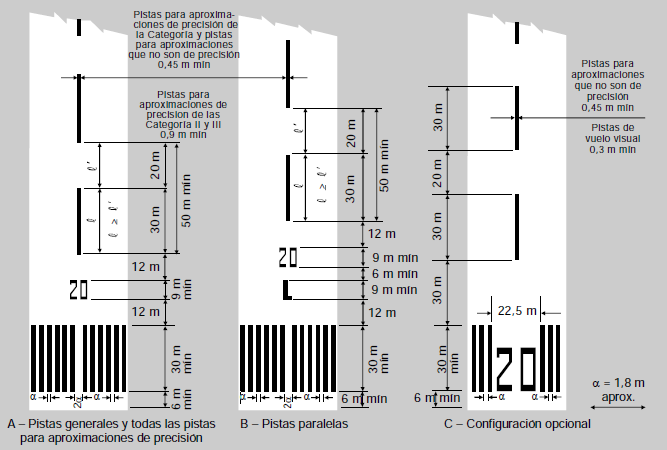
\includegraphics[clip, trim=0cm 0cm 0cm 0cm, width=0.911\textwidth]{./images/markings/centreline}
			\caption{Centreline according to ICAO's recommendations.} %nom de la figura
			\label{} %per denotar una referencia
		\end{figure}
	
		Due to the fact that the airport has two parallel runways, the model used will be the middle one. 
		
		The following figure attached will be shown as an example:
		
		\begin{figure}[H]
			\centering
			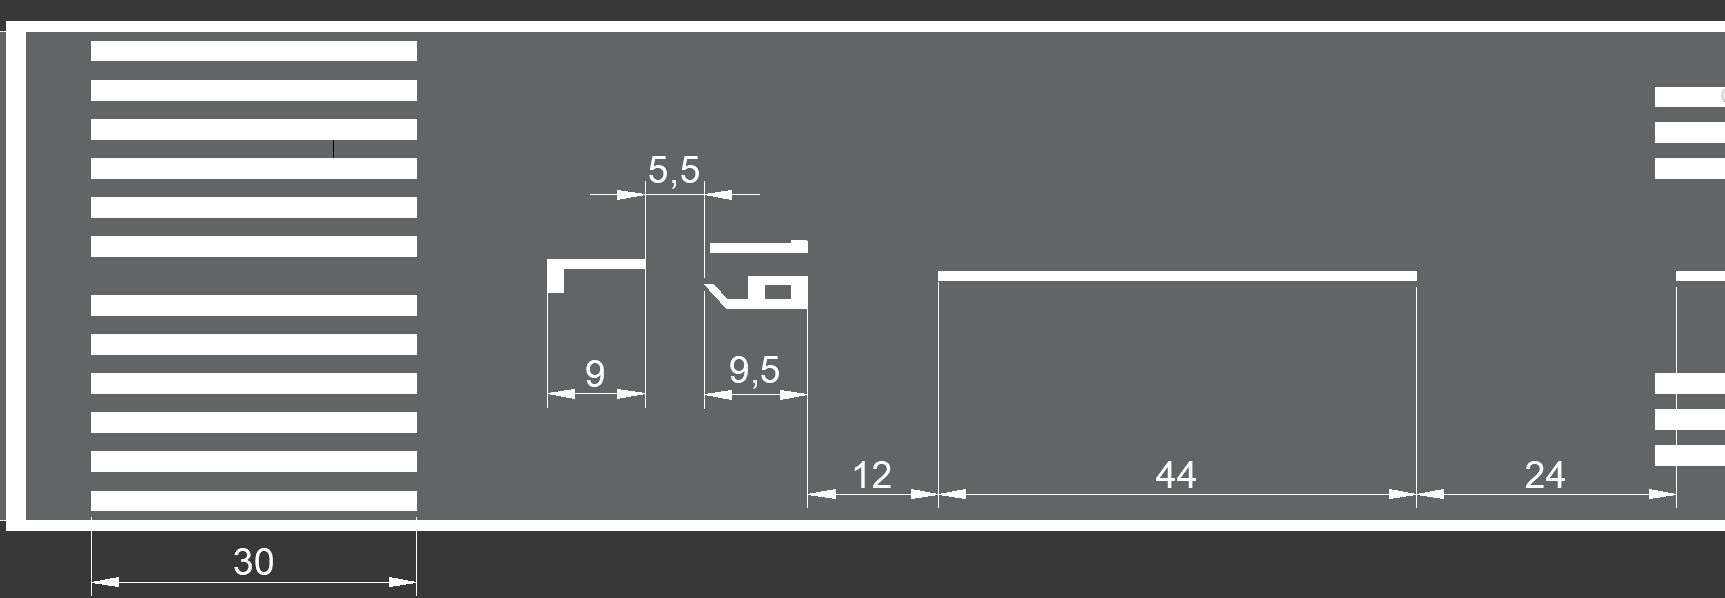
\includegraphics[clip, trim=0cm 0cm 0cm 0cm, 	width=0.911\textwidth]{./images/markings/centreexample}
			\caption{Centre line of the international runway.} %nom de la figura
			\label{} %per denotar una referencia
		\end{figure}
		
		\subsection{Runway's threshold markings}
		\paragraph{}The strips that indicate the start of the threshold will start at 6 m from the beginning of the threshold, and will contain 12 stripes, choosing the configuration specified in the Annex 14 part 5.2.4.6., including a minimum of 30m of length and 1,80m of width, with a separation of approximately 1,80m.
		
		\subsubsection{Arrows}
		\paragraph{}The runway's aiming point markings will be placed if the threshold is displaced from the runway extreme. As in the case of the Bekasi-East Jakarta both runways (4E and 4C) the threshold will be displaced, they are a must. They will be coloured in white.
		
		\begin{figure}[H]
			\centering
			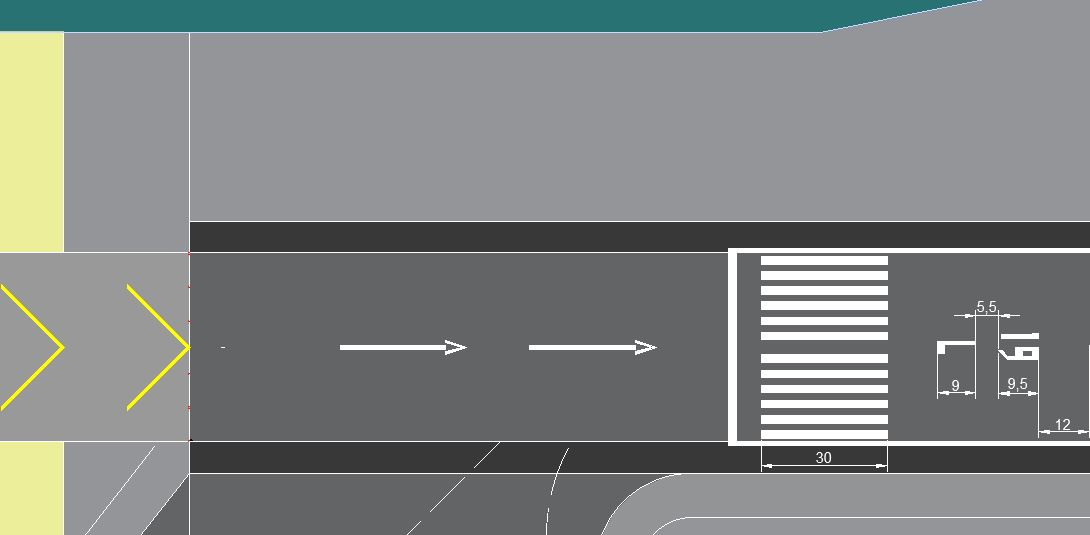
\includegraphics[clip, trim=0cm 0cm 0cm 0cm, 	width=0.911\textwidth]{./images/markings/arrows}
			\caption{Example of arrows pointing at the threshold.} %nom de la figura
			\label{} %per denotar una referencia
		\end{figure}
		
		\subsection{Runway's designation marking}
		\paragraph{}It will be placed in the threshold and in the case of Jakarta airport will be mandatory in all the cases as they all are paved. This designer will consist in two numbers referred to the azimuthal position. This number will be accompanied by a letter, indicating the order of appearance. 
		
		
		\subsection{Runway's aiming point markings}
		\paragraph{}As both runways meet the criteria, an aiming point is needed. The following table extracted from the annex 14 will show us which parameters should the aiming point mark have depending on the runway's category: 
		
		\begin{figure}[H]
			\centering
			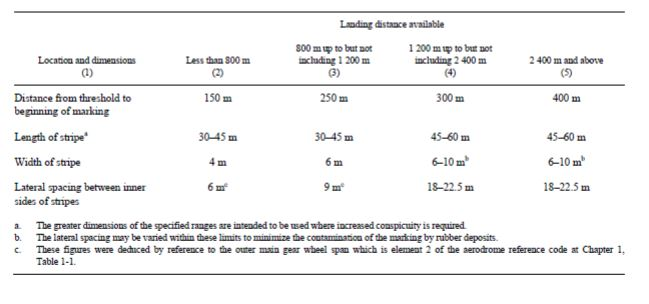
\includegraphics[clip, trim=0cm 0cm 0cm 0cm, 	width=0.8\textwidth]{./images/markings/aimpointtable}
			\caption{Table gathering all the aiming point marking parameters.} %nom de la figura
			\label{} %per denotar una referencia
		\end{figure}
		
		So, since both runways have a RFL higher than 2400m, the distance between the threshold and the start of the marking will be at 400 m, with a length of 60 m, a width of 10 m and a separation of 18 m. The following figure may serve as an example:
		
		\begin{figure}[H]
			\centering
			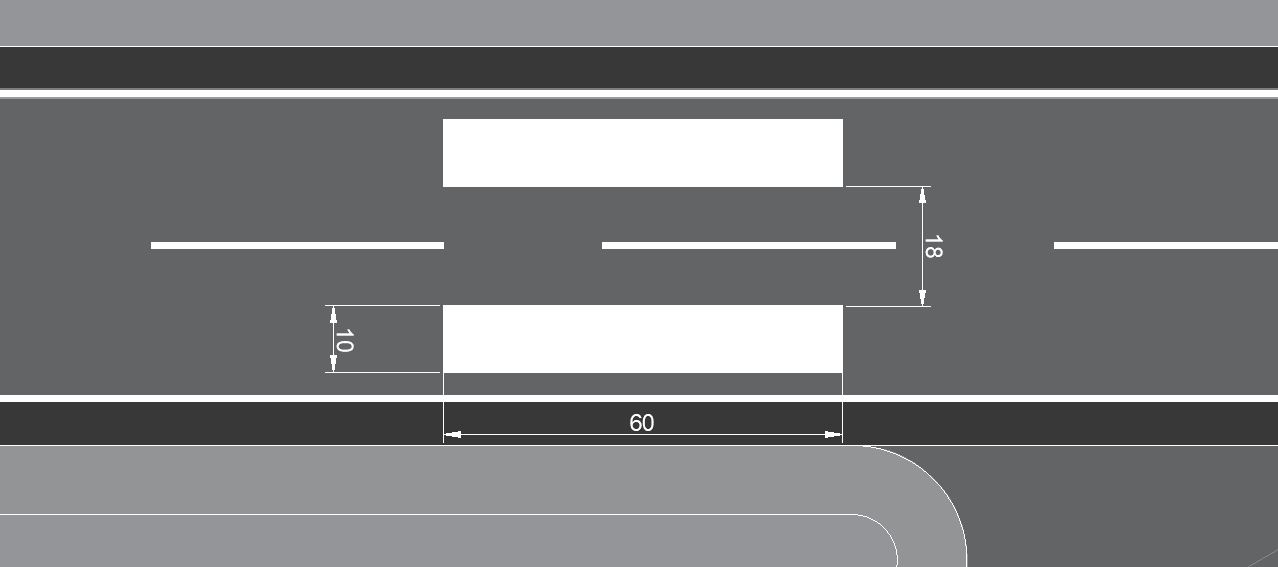
\includegraphics[clip, trim=0cm 0cm 0cm 0cm, 	width=0.911\textwidth]{./images/markings/aimpoint}
			\caption{Example of aiming point markings placed in runway 1.} %nom de la figura
			\label{} %per denotar una referencia
		\end{figure}
		
	\section{Taxiway's and holding position's markings}
		\subsection{Introduction}
		\paragraph{}Due to the fact that the airport being designed is a 4-type for both runways, the markings in the taxiways will be mandatory. The axis will be projected respecting the distances when curves appear and respecting the established hierarchy, that is to say, keeping in mind that they are subordinated to runways. The dimensions of this marking will be continuous and with 15cm of width at least, except in the event of an intersection.
		
		\subsection{Runway's entry holding position markings}
		The runway's entry holding position markings will be directly painted in the AutoCAD model following the regulations and recommendations stated in the annex 14.
				
		\subsection{Mandatory instruction markings}
		\paragraph{}If there is no possibility of positioning a sign with mandatory indications, this indication will be painted in the pavement. In the case of the type C runway, this signal will be centred in the middle of the centreline, interrupting it, whereas in the type F runway the signal will be placed twice on each side of the axis. 
		
		The characters will be painted in white with a red background and the height of the different characters should be of, at least, 4m.
		
		\begin{figure}[H]
			\centering
			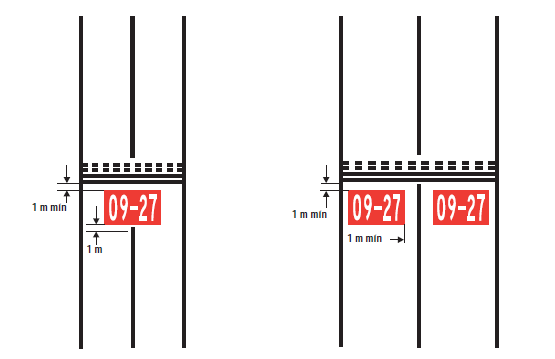
\includegraphics[clip, trim=0cm 0cm 0cm 0cm, 	width=0.911\textwidth]{./images/markings/mandatorymarks}
			\caption{Design used in order to define the mandatory instruction markings.} %nom de la figura
			\label{} %per denotar una referencia
		\end{figure}
	
		\subsection{Information markings}
		\paragraph{}Depending of the information given, the colours of the information markings will be:
		
		-	Yellow characters with black background if it gives emplacement information.
		
		-	Black background with yellow background if it gives direction or destiny information.
	
	\section{Apron's markings} 
		\subsection{Introduction}
		\paragraph{}They will include the identification number of every lot, with its guideline, alignment guide, stop line and departure line. The markings should be represented bearing in mind that the pilot should also be able to see the markings from the cabin. The guidelines should also be continuous with a width of, at least, 15cm, like the width of the alignment line in the final parking position.

		\subsection{Stand safety lines markings}
		\paragraph{}When considered necessary, the platform surface may include a safe separation distance between the different aircraft, such as wing tip margin lines. They will be continuous with a width of, at least, 10cm.

		
	